\documentclass{article}
%%%%%%%%%%%%%%%%%%%%%%%%%%%%%%%%%%%%%%%%%%%%%%%%%%%%%%%%%%%%%%%%%%%%%%%%%%%%%%%%%%%%%%%%%%%%%%%%%%%%%%%%%
\usepackage{csquotes,xpatch}% recommended
\usepackage[backend=bibtex,
style=authoryear-comp,
sortcites=false,
maxbibnames=5,maxcitenames=2,
firstinits=true,
natbib=true,
]{biblatex}

\addbibresource{refs.bib}

% natbib = true: add comma between author and year
% firstinits: for first name initials in bibliography
\renewcommand{\postnotedelim}{ } % remove comma in post citation in autocite
%\addbibresource{refs.bib}
%%%%%%%%%%%%%%%%%%%%%%%%%%%%%%%%%%%%%%%%%%%%%%%%%%%%%%%%%%%%%%%%%%%%%%%%%%%%%%%%%%%%%%%%%%%%%%%%%%%%%%%%%

% Combine label and labelyear links
\xpatchbibmacro{cite}
{\usebibmacro{cite:label}%
	\setunit{\addspace}%
	\usebibmacro{cite:labelyear+extrayear}}
{\printtext[bibhyperref]{%
		\DeclareFieldAlias{bibhyperref}{default}%
		\usebibmacro{cite:label}%
		\setunit{\addspace}%
		\usebibmacro{cite:labelyear+extrayear}}}{}{}

% Include labelname in labelyear link
\xpatchbibmacro{cite}
{\printnames{labelname}%
	\setunit{\nameyeardelim}%
	\usebibmacro{cite:labelyear+extrayear}}
{\printtext[bibhyperref]{%
		\DeclareFieldAlias{bibhyperref}{default}%
		\printnames{labelname}%
		\setunit{\nameyeardelim}%
		\usebibmacro{cite:labelyear+extrayear}}}{}{}

% Access hyperref's citation link start/end commands
\makeatletter
\protected\def\blx@imc@biblinkstart{%
	\@ifnextchar[%]
	{\blx@biblinkstart}
	{\blx@biblinkstart[\abx@field@entrykey]}}
\def\blx@biblinkstart[#1]{%
	\blx@sfsave\hyper@natlinkstart{\the\c@refsection @#1}\blx@sfrest}
\protected\def\blx@imc@biblinkend{%
	\blx@sfsave\hyper@natlinkend\blx@sfrest}
\blx@regimcs{\biblinkstart \biblinkend}
\makeatother

\newbool{cbx:link}

% Include parentheses around labelyear in \textcite only in
% single citations without pre- and postnotes
\def\iflinkparens{%
	\ifboolexpr{ test {\ifnumequal{\value{multicitetotal}}{0}} and
		test {\ifnumequal{\value{citetotal}}{1}} and
		test {\iffieldundef{prenote}} and
		test {\iffieldundef{postnote}} }}

\xpatchbibmacro{textcite}
{\printnames{labelname}}
{\iflinkparens
	{\DeclareFieldAlias{bibhyperref}{default}%
		\global\booltrue{cbx:link}\biblinkstart%
		\printnames{labelname}}
	{\printtext[bibhyperref]{\printnames{labelname}}}}{}{}

\xpatchbibmacro{textcite}
{\usebibmacro{cite:label}}
{\iflinkparens
	{\DeclareFieldAlias{bibhyperref}{default}%
		\global\booltrue{cbx:link}\biblinkstart%
		\usebibmacro{cite:label}}
	{\usebibmacro{cite:label}}}{}{}

\xpretobibmacro{textcite:postnote}
{\ifbool{cbx:link}% patch 2.7+
	{\ifbool{cbx:parens}
		{\bibcloseparen\global\boolfalse{cbx:parens}}
		{}%
		\biblinkend\global\boolfalse{cbx:link}}
	{}}
{}
{\xpatchbibmacro{textcite}% patch earlier releases
	{\setunit{%
			\ifbool{cbx:parens}
			{\bibcloseparen\global\boolfalse{cbx:parens}}
			{}%
			\multicitedelim}}
	{\ifbool{cbx:link}
		{\ifbool{cbx:parens}
			{\bibcloseparen\global\boolfalse{cbx:parens}}
			{}%
			\biblinkend\global\boolfalse{cbx:link}}
		{}%
		\setunit{%
			\ifbool{cbx:parens}
			{\bibcloseparen\global\boolfalse{cbx:parens}}
			{}%
			\multicitedelim}}
	{}{}}
%%%%%%%%%%%%%%%%%%%%%%%%%%%%%%%%%%%%%%%%%%%%%%%%%%%%%%%%%%%%%%%%%%%%%%%%%%%%%%%%%%%%%%%%%%%%%%%%%%%%%%%%%
\DeclareNameAlias{sortname}{last-first} % last name first
\renewbibmacro{in:}{} % remove in: before journal

%%%%%%%%%%%%%%%%%%%%%%%%%%%%%%%%%%%%%%%%%%%%%%%%%%%%%%%%%%%%%%%%%%%%%%%%%%%%%%%%%%%%%%%%%%%%%%%%%%%%%%%%%
\usepackage{graphicx}
\usepackage{epstopdf} 
%%%%%%%%%%%%%%%%%%%%%%%%%%%%%%%%%%%%%%%%%%%%%%%%%%%%%%%%%%%%%%%%%%%%%%%%%%%%%%%%%%%%%%%%%%%%%%%%%%%%%%%%%
\usepackage{calrsfs}
\usepackage{physics}
\usepackage{mathtools}  
\usepackage{amsmath}
\usepackage{amssymb}
\usepackage{tabulary}
\usepackage{booktabs}
\usepackage{hyperref}
%%%%%%%%%%%%%%%%%%%%%%%%%%%%%%%%%%%%%%%%%%%%%%%%%%%%%%%%%%%%%%%%%%%%%%%%%%%%%%%%%%%%%%%%%%%%%%%%%%%%%%%%%
%\usepackage{chngcntr}
%\numberwithin{equation}{chapter}
%\counterwithin{figure}{chapter}
%%%%%%%%%%%%%%%%%%%%%%%%%%%%%%%%%%%%%%%%%%%%%%%%%%%%%%%%%%%%%%%%%%%%%%%%%%%%%%%%%%%%%%%%%%%%%%%%%%%%%%%%%
\setlength{\parindent}{2em}
\setlength{\parskip}{1em}

\linespread{1.6}
\usepackage{geometry}
\geometry{
	a4paper,
	total={134mm,225mm},
	left=38mm,
	top=35mm,
	headsep=.5in
}
\raggedbottom
%%%%%%%%%%%%%%%%%%%%%%%%%%%%%%%%%%%%%%%%%%%%%%%%%%%%%%%%%%%%%%%%%%%%%%%%%%%%%%%%%%%%%%%%%%%%%%%%%%%%%%%%%
\usepackage{blindtext}
\usepackage{ragged2e}
\usepackage{float}

\usepackage{epstopdf}
\usepackage{empheq} 

\usepackage{array}
\hypersetup{
	colorlinks
}
%%%%%%%%%%%%%%%%%%%%%%%%%%%%%%%%%%%%%%%%%%%%%%%%%%%%%%%%%%%%%%%%%%%%%%%%%%%%%%%%%%%%%%%%%%%%%%%%%%%%%%%%%
\usepackage{graphics}
\graphicspath{ {figures/} }
\renewcommand{\listfigurename}{List of figures}

\usepackage[labelfont=bf,justification=justified,singlelinecheck=false]{caption}
\captionsetup[figure]{name=Fig. ,labelsep=period}
\captionsetup[table]{labelsep=period}
\captionsetup[figure]{labelfont={bf},labelformat={default},labelsep=period,name={Fig.}}
%%%%%%%%%%%%%%%%%%%%%%%%%%%%%%%%%%%%%%%%%%%%%%%%%%%%%%%%%%%%%%%%%%%%%%%%%%%%%%%%%%%%%%%%%%%%%%%%%%%%%%%%%
\usepackage{array}
\usepackage{longtable}
\usepackage{xcolor}

\usepackage{comment}

\usepackage{enumitem}

\usepackage{wrapfig}
%%%%%%%%%%%%%%%%%%%%%%%%%%%%%%%%%%%%%%%%%%%%%%%%%%%%%%%%%%%%%%%%%%%%%%%%%%%%%%%%%%%%%%%%%%%%%%%%%%%%%%%%%
\usepackage{titlesec}

\titlespacing*{\section}
{0pt}{1ex plus .5ex minus .2ex}{.5ex plus .2ex}
\titlespacing*{\subsection}
{0pt}{0.5ex plus .5ex minus .2ex}{.5ex plus .2ex}
%\titlespacing*{\subparagraph}
%{0pt}{2.5ex plus 1ex minus .2ex}{1.3ex plus .2ex}

\setcounter{secnumdepth}{4}
\setcounter{tocdepth}{4}

\newcommand{\hsp}{\hspace{5pt}}

\titleformat{\section}[block]{\bfseries\large}{\thesection}{1em}{}
\titleformat{\subsection}[block]{\bfseries\itshape}{\thesubsection}{1em}{}


%\titleformat{\subsubsection}
%{\normalfont\normalsize\itshape}{\thesubsubsection}{1em}{}
%\titleformat{\subparagraph}[runin]
%{\itshape\normalsize}{\thesubparagraph}{1em}{}

%%%%%%%%%%%%%%%%%%%%%%%%%%%%%%%%%%%%%%%%%%%%%%%%%%%%%%%%%%%%%%%%%%%%%%%%%%%%%%%%%%%%%%%%%%%%%%%%%%%%%%%%%
\usepackage{subcaption}
\usepackage{bbm}
\usepackage{tabularx}
%%%%%%%%%%%%%%%%%%%%%%%%%%%%%%%%%%%%%%%%%%%%%%%%%%%%%%%%%%%%%%%%%%%%%%%%%%%%%%%%%%%%%%%%%%%%%%%%%%%%%%%%%
\definecolor{mycolor}{RGB}{207,42,40}
\AtBeginDocument{\hypersetup{citecolor=violet, linkcolor = mycolor}}

\usepackage{indentfirst}


%%%%%%%%%%%%%%%%%%%%%%%%%%%%%%%%%%%%%%%%%%%%%%%%%%%%%%%%%%%%%%%%%%%%%%%%%%%%%%%%%%%%%%%%%%%%%%%%%%%%%%%%
\setlength{\belowcaptionskip}{-20pt}


\usepackage{enumitem}
\usepackage{amsmath,bm}
\usepackage{graphicx}

\DeclareMathAlphabet{\pazocal}{OMS}{zplm}{m}{n}

\usepackage[ruled,vlined]{algorithm2e}
\SetKwComment{Comment}{$\triangleright$\ }{}
\newenvironment{problem_algorithm}[1][htb]
{\renewcommand{\algorithmcfname}{Algorithm for Problem}% Update algorithm name
	\begin{algorithm}[#1]%
	}{\end{algorithm}}

\usepackage{hyperref}

\begin{document}
	
	\sloppy
	
%%%%%%%%%%%%%%%%%%%%%%%%%%%%%%%%%%%%%%%%%%%%%%%%%%%%%%%%%%%%%%%%%%%%%%%%%%%%%%%%%%%%%%%%%%%%%%%%%%%%%%%%%
	\begin{center}	
		\Large
		\textbf{Meta-learning / meta architecture search / PINNs}\\
		\large
%		\today
	\end{center}
	\vskip 0.5in
	
%%%%%%%%%%%%%%%%%%%%%%%%%%%%%%%%%%%%%%%%%%%%%%%%%%%%%%%%%%%%%%%%%%%%%%%%%%%%%%%%%%%%%%%%%%%%%%%%%%%%%%%%%
{\footnotesize
	\setlength{\parskip}{0.1em}
	\linespread{0.1}
	\tableofcontents}

\newpage
\section{Motivation}\label{sec:motivation}
\begin{itemize}
	\item We are interested in the following problems:
	\begin{enumerate}[font={\bfseries},label={Problem (\arabic*):}]
		\item Obtaining a well-performing set of hyperparameters for solving a specific task. Examples include:
		\begin{itemize}
			\item Fitting a regression curve to a given dataset; what's the best architecture?
			\item Solving a PDE with a fixed set of PDE parameters (PINNs); what's the best loss function to use?
			\item Using B-PINNs for obtaining a stochastic solution to a deterministic PDE; what's the best prior parameters?
		\end{itemize}
		\item Obtaining a well-performing set of hyperparameters such that if used for solving an arbitrary unseen task it will perform well. 
		We assume that this new task is a sample from a task distribution that we have samples from. 
		You may see it as few-shot/iterations learning in the literature.
		Examples include:
		\begin{itemize}
			\item New task will be given by $f(x) = sin(\lambda x)$ where $\lambda \in Uniform([0, 1])$. 
			Find the architecture that will perform best if used for fitting data corresponding to a new $\lambda$ value.
			\item New PDE will be given by $\lambda \partial_x^2 u - u = f(x)$ where $f$ is known and $\lambda \in Uniform([0, 1])$.
			Find the loss function that will produce the most accurate $u(x)$ if used in conjunction with PINNs for a new $\lambda$ value.
			\item New PDE will be given as above.
			Assuming a Gaussian prior for the parameters of the fitting NN, find the prior standard deviation such that if used in conjunction with B-PINNs for a new $\lambda$ value it will produce the most accurate $u(x)$.
			This means that tasks \textit{share the prior} and given a new task we still have to do posterior approximation! 
			But hopefully it will be faster and/or more accurate. 
		\end{itemize}
		\item Finding a way to optimize hyperparameters efficiently for a new task. 
		You may see it as few-shot/iterations meta-learning in the literature.
		Examples include:
		\begin{itemize}
			\item For a new regression task (new $\lambda$) we want to make architecture search efficient. This means that tasks \textit{do not share} some obtained architecture but \textit{use the same techniqu}e for finding it. Therefore, we get a task-specific optimal architecture! 
			\item For a new PDE we want to make loss function optimization efficient. Tasks do not share the same loss function but use the same technique for optimizing it. We get a \textit{task-specific optimal loss function}! 
		\end{itemize}
	\end{enumerate}
\end{itemize}

\section{General meta-learning formulation}
\begin{itemize}
	\item \textbf{Problems (1)} and \textbf{(2)} are considered first. 
	See Section~\ref{sec:problem:3} for \textbf{Problem (3)}.
	\item Meta-training is commonly formalized as follows:
	\begin{equation}
		\begin{aligned}
			\min_{x} \pazocal{L}_1(y^*(x), x) \\
			\text{s.t. } y^*(x) = argmin_y \pazocal{L}_2(y, x) \\
			\text{i.e., for GD: } y^*(x) = y_0(x) - \sum_{j=1}^{J}\epsilon_2 g_j(x, y_{j-1})
		\end{aligned}
	\end{equation}
	\item This is called bi-level optimization: note that $x$ and $y$ are not optimized together.
	\item $x$ denotes hyperparameters to be optimized and $y$ the NN parameters.
	\item $\pazocal{L}_1$ is the meta-objective (or outer), $\pazocal{L}_2$ is the base-learning objective (or lower or inner).
	\begin{enumerate}
		\item For \textbf{Problem (1)}:
		\begin{equation}\label{eq:problem:1:losses}
			\begin{aligned}
				\pazocal{L}_1(y^*(x), x) = \mathbb{E}_{D_{val}} \pazocal{L}(y^*(x), x) \\
				\pazocal{L}_2(y, x) = \mathbb{E}_{D_{train}} \pazocal{L}(y, x)
			\end{aligned}
		\end{equation}
		\item For \textbf{Problem (2)}:
		\begin{equation}\label{eq:problem:2:losses}
			\begin{aligned}
				y^*(x) = \{y^*_{task}\}_{tasks}\\
				\pazocal{L}_1(y^*(x), x) = \mathbb{E}_{tasks}\mathbb{E}_{D_{val, task}} \pazocal{L}(y^*_{task}(x), x) \\
				\pazocal{L}_2(y, x) = \mathbb{E}_{D_{train, task}} \pazocal{L}(y, x)
			\end{aligned}
		\end{equation}
	\end{enumerate}
	\item $\mathbb{E}_{D}\pazocal{L}(y, x)$ is the average loss over the data defined by $D$ (e.g., squared error) evaluated on the NN parameters $y$. It may depend on $x$ (e.g., parametrized loss function). 
	\item Based on this formulation, \textbf{Problem (1)} is a special case of \textbf{Problem (2)}; just one task is considered and we ``meta-overfit'' on this task: most likely the obtained optimal hyperparameters cannot be transferred for solving other tasks.
\end{itemize}

\section{Placing 4 meta-learning techniques under the general formulation}
\subsection{NAS-DARTS}

\begin{center}
	\begin{tabular}{ | c || c |} 
		\hline
		$x$ & architecture parameters \\
		\hline
		$y$ & NN parameters \\
		\hline
		$y^*(x)$ & optimal NN parameters corresponding to architecture defined by $x$ \\
		\hline
	\end{tabular}
\end{center}
\begin{itemize}
	\item As defined originally by \textcite{liu2019darts}, it solves \textbf{Problem (1)}: finds best architecture for solving a specific task.
	\item One inner optimization step is typically used ($J = 1$).
	\item $y_0(x) = y^*$ of previous iteration: we start with an architecture, we update weights, then we update architecture, and then update weights again.
	\item For regression, $\pazocal{L}_1$ is the MSE on the validation data and $\pazocal{L}_2$ the MSE on the training data.
	\item $\pazocal{L}_1$ \textbf{does depend} explicitly on $x$.
	We take total derivative $\frac{d}{dx}\pazocal{L}_1(y^*(x), x)$ for updating $x$, so this is important.
	\item When done, NN parameters need retraining because the architecture is hard-pruned.
\end{itemize}

\subsection{Prior optimization - Empirical Bayes}

\begin{center}
	\begin{tabular}{ | c || c |} 
		\hline
		$x$ & prior parameters \\
		\hline
		$y$ & posterior parameters \\
		\hline
		$y^*(x)$ & optimal posterior parameters corresponding to prior defined by $x$ \\
		\hline
	\end{tabular}
\end{center}
\begin{itemize}
	\item It solves \textbf{Problem (1)}: finds best prior for solving a specific task.
	\item One inner optimization step is typically used ($J = 1$).
	\item $y_0(x) = y^*$ of previous iteration: we start with a prior, we update posterior parameters, then we update prior, and then update posterior again.
	\item For VI, $\pazocal{L}_1$ and $\pazocal{L}_2$ are the ELBO on the training data (usually no validation data is used - check).
	\item $\pazocal{L}_1$ \textbf{does depend} explicitly on $x$.
	\item When done, posterior parameters can be used as they are. No need for retraining using the obtained prior.
\end{itemize}

\subsection{MAML}

\begin{center}
	\begin{tabular}{ | c || c |} 
		\hline
		$x$ & initial NN parameters \\
		\hline
		$y$ & NN parameters \\
		\hline
		$y^*(x)$ & optimal NN parameters \\
		\hline
	\end{tabular}
\end{center}
\begin{itemize}
	\item As defined originally by \textcite{finn2017modelagnostic}, it solves \textbf{Problem (2)}: finds best initial parameters such that if used for a new learning task final parameters will be obtained fast and be well-performing.
	\item One inner optimization step is used ($J = 1$) but it is performed for every task.
	\item $y_0(x) = x$: note the difference!
	\item For regression, $\pazocal{L}_1$ and $\pazocal{L}_2$ are the mean MSE on randomly sampled data from randomly sampled tasks.
	\item $\pazocal{L}_1$ \textbf{does not depend} explicitly on $x$.
\end{itemize}

\subsection{Loss function meta-learning}
\begin{center}
	\begin{tabular}{ | c || c |} 
		\hline
		$x$ & loss function parameters \\
		\hline
		$y$ & NN parameters \\
		\hline
		$y^*(x)$ & optimal NN parameters \\
		\hline
	\end{tabular}
\end{center}
\begin{itemize}
	\item As defined originally by \textcite{bechtle2020metalearning}, it solves \textbf{Problem (2)}: finds best loss function parameters such that if used for a new learning task final parameters will be obtained fast and be well-performing.
	\item One or more inner optimization steps are used ($J = 1$) and are performed for one task.
	\item $y_0(x)$ is randomly initialized. 
	\item For regression, $\pazocal{L}_1$ is the MSE on randomly sampled data from the selected task and $\pazocal{L}_2$ is the \textit{learned loss function} on randomly sampled data from the selected task.
	\item Selected task can change after a few iterations. 
	\item $\pazocal{L}_1$ \textbf{does not depend} explicitly on $x$.
\end{itemize}

\section{Making task-specific techniques (Problem 1) be task-agnostic (Problem 2)}\label{sec:making:agnostic}
\begin{itemize}
\item Based on Eqs.~\eqref{eq:problem:1:losses}-\eqref{eq:problem:2:losses}, for making a task-specific technique be task-agnostic we have to perform the inner-optimization for every task separately, obtain $y^*_{task}(x)$ for every task and then update $x$ based on the average performance of the $y^*_{task}(x)$ values.

\item Practically, this means that we can use NAS-DARTS to find an optimal architecture for a set of tasks. 
This is what Auto-Meta (\cite{kim2018autometa}) does, but they use PNAS instead of DARTS for architecture search.

\begin{itemize}
	\item Has it been done for NAS-DARTS?
\end{itemize}
\item Can we obtain also a good initialization for this shared architecture? It's not too hard to combine NAS and MAML (we can update architecture and initialization together in the outer loop).
\begin{itemize}
	\item Inner loop: Update parameters based on current architecture and current initial parameters
	\item Outer update: Update architecture and initial parameters simultaneously
\end{itemize}
\item Auto-MAML (\cite{lian2019fast}) is a variant of the above (algorithm p. 15 - algorithm in the paper has typos - check):
\begin{itemize}
	\item Inner loop 1: Update parameters based on current architecture and current initial parameters
	\item Outer update 1: Update initial parameters as we do in MAML
	\item Inner loop 2: Update parameters based on current architecture and current initial parameters
	\item Outer update 2: Update architecture as we do in DARTS
\end{itemize}

\item The only problem is that the NAS-obtained architecture needs to be sparsified before using it. So how good are the obtained initial parameters if we hard-prune the architecture after meta-training? Look in \textcite{elsken2020metalearning} (Section 4) for the solution they propose regarding this.

\item Another instance of making task-specific techniques (\textbf{Problem 1}) be task-agnostic (\textbf{Problem 2}) would be to find a good prior that performs well for a distribution of tasks and not only for a single task.
\end{itemize}

\section{Addressing Problem (3)}\label{sec:problem:3}
\begin{itemize}
	\item It can be addressed as a combination of \textbf{Problems (1)} and \textbf{(2)}: Obtain a well-performing set of hyperparameters such that if used for some other hyperparameter optimization for an unseen task it will perform well.
	\item \textbf{Example:} Find some initial architecture that with only a few optimization/adaptation steps can become optimal for an unseen task.
	This is done by combining NAS-DARTS with MAML: Recall that in MAML we look for optimal initialization. Here we optimize architecture and NN parameters together and we look for a good initialization of both.
	
	\begin{center}
		\begin{tabular}{ | c || c |} 
			\hline
			$x$ & initial architecture and corresponding parameters \\
			\hline
			$y$ & architecture and corresponding parameters \\
			\hline
			$y^*(x)$ & optimal architecture and corresponding parameters \\
			\hline
		\end{tabular}
	\end{center}
	\item This is what T-NAS (transferable NAS) does (\cite{lian2019fast}).
	Recall however that both NAS and MAML are two-step procedures. 
	Thus, the above requires 3 steps which increases the computational cost.
	This is why \textcite{lian2019fast} propose to reduce NAS into a single step (weights are updated simultaneously with architecture). 
	However, this is something that the original NAS authors (\cite{liu2019darts} - Section 3.3) suggest to avoid because it leads to overfitting the architecture (we have exactly the same problem if we optimize prior and posterior simultaneously).
	\item In summary, this is T-NAS:
	\begin{itemize}
		\item In meta-train time, it finds a good architecture and parameter initialization
		\item In meta-test time, it quickly optimizes architecture and parameters with standard NAS (architecture is still continuous)
		\item Then architecture is pruned
		\item Finally, model is retrained with pruned architecture
	\end{itemize}
	Inner loop for each task $i$ ($\theta_i^0 = \tilde{\theta}$ and $w_i^0 = \tilde{w}$):
	\setlength{\belowcaptionskip}{-40pt}
	\begin{figure}[H]
		\centering
		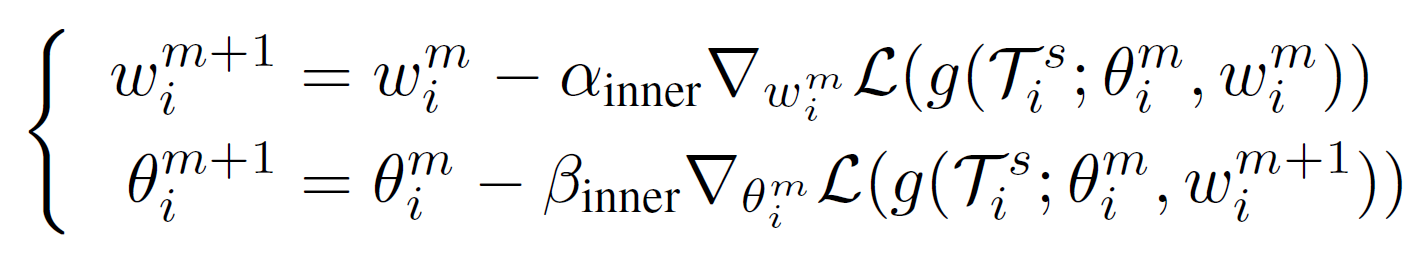
\includegraphics[width=.55\linewidth]{./figs/meta_nas_inner.png}  
		\caption*{}
		%\label{fig:lr_sched}
	\end{figure}
	Outer update:
	\begin{figure}[H]
		\centering
		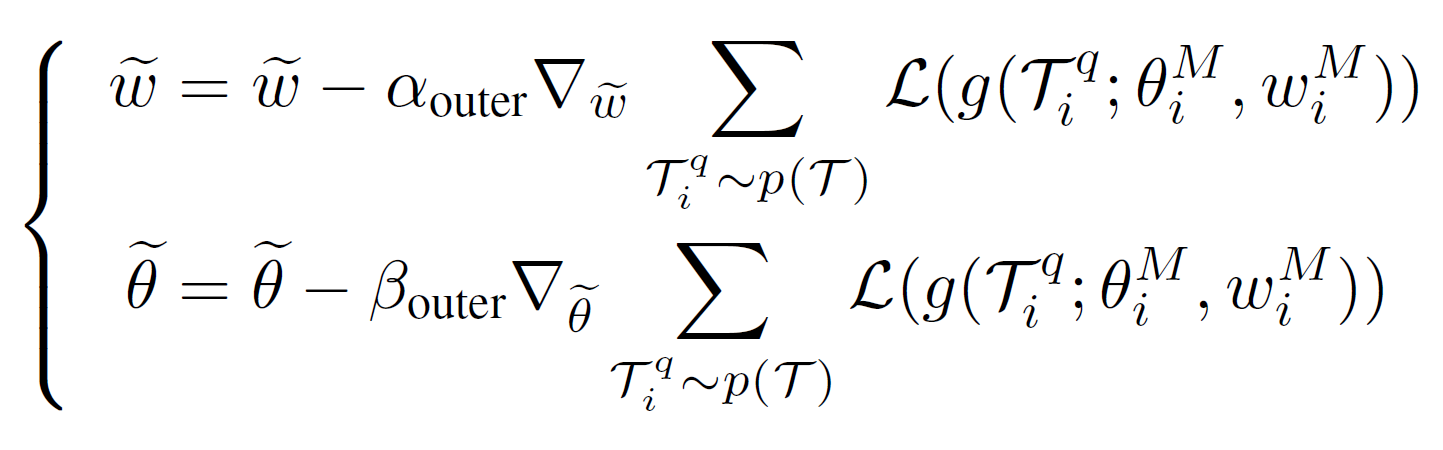
\includegraphics[width=.5\linewidth]{./figs/meta_nas_outer.png}  
		\caption*{}
		%\label{fig:lr_sched}
	\end{figure}
	\item Clearly, having to retrain after pruning poses a computational cost limitation.
	\item \textcite{elsken2020metalearning} addresses this issue by using soft-pruning: their technique is called Meta-NAS.

\end{itemize}

\section{Bayesian way for addressing Problem (3)}
This is ``meta architecture search'' as proposed by \textcite{shaw2019meta}.
Let's incorporate it into our general framework. 
First, we discuss Bayesian NAS which aims to solve \textbf{Problem (1)} (seems to be what BayesNAS in \cite{zhou2019bayesnas} does - check) and then we discuss the technique of \textcite{shaw2019meta} which aims to solve \textbf{Problem (3)}, but is essentially based on Bayesian NAS.
\subsection{Bayesian NAS}
\begin{itemize}
	\item A first step towards a Bayesian variant of NAS is to replace the two-step optimization of NAS by one step: optimize $x$ (architecture) and $y$ (NN parameters) simultaneously. 
	Once again, this leads to overfitting for the deterministic case (\cite{liu2019darts}).
	\item Next, since this is a simple optimization we can make it Bayesian: instead of looking for the best pair [architecture, parameters] we look for their posterior. 
	The best pair [architecture, parameters] corresponds to the maximum posterior probability. 
	\item After obtaining the posterior we can sample from it and use the obtained pair [architecture, parameters] as the predictive model.
	\item In summary, not only we have obtained the best architecture but we have also trained it.
	And by sampling the posterior we also have its uncertainty.
	\item In standard Bayesian framework a sample from the parameter posterior is used in the only architecture we have in order to obtain a sample prediction. 
	In Bayesian NAS a sample from the posterior gives us both an architecture and its optimal parameters and we get a sample prediction by evaluating the architecture on these parameters.
\end{itemize}

\subsection{Meta architecture search}
\begin{itemize}
	\item For an unseen task we want to perform Bayesian NAS efficiently.
	\item In other words, we want to obtain a prior for Bayesian NAS that works well for many tasks.
	\item Inner loop: perform Bayesian NAS for all tasks \textbf{separately} with fixed prior. 
	Obtain one posterior of [architecture, parameters] for each task. 
	\item Outer update: Update prior based on the performance of obtained posteriors towards maximizing average (across tasks) ELBO.	
\end{itemize}

\section{General algorithms}\label{sec:}

\begin{problem_algorithm}[H]
	\label{algo:problem:1}
	\SetAlgoLined
	\textbf{input:} $\epsilon_1$, $\epsilon_2$, $\pazocal{L}_1$, $\pazocal{L}_2$ and task data
	
	initialize $x$ with $x_0$ 
	\Comment*[f]{also $y^*_{0}$ if needed (e.g., in NAS-DARTS)}
	
	\For{$i \in \{1,\dots, I\}$}{
		initialize $y$ with $y_0$
		\Comment*[f]{
			$y_0 = y_0(x_{i-1})$ or $y_0(y^*_{i-1})$}
		
		\For{$j \in \{1,\dots, J\}$}{
			$y_j = y_{j-1} - \epsilon_2 \nabla_y\pazocal{L}_2(y,x)\bigg\rvert_{y = y_{j-1}, \ x = x_{i-1}}$
			\Comment*[f]{Inner step}			
		}
		set $y^*_i = y_J$ \Comment*[f]{for GD: $y^*_i = y_0 - \sum_{j=1}^{J}\epsilon_2 g_j(y_{j-1}, x_{i-1})$}
		
		$x_i = x_{i-1} - \epsilon_1 \boldsymbol{d}_x\pazocal{L}_1(y^*(x),x)\bigg\rvert_{y^* = y^*_i, \ x = x_{i-1}}$	 \Comment*[f]{Outer step}	
	}
	
	\textbf{return} $x_I$ and $y^*_I$
	\caption{Good hyperparameters for a specific task}
\end{problem_algorithm}

\begin{problem_algorithm}[H]
	\label{algo:problem:2}
	\SetAlgoLined
	\textbf{input:} $\epsilon_1$, $\epsilon_2$, $\pazocal{L}_1$, $\pazocal{L}_2$ and task distribution $p(\pazocal{T})$
	
	initialize $x$ with $x_0$ 
	
	\For{$i \in \{1,\dots, I\}$}{
		sample $T$ tasks from $p(\pazocal{T})$
		
		\For{$\tau \in \{1,\dots, T\}$}{
			initialize $y^{(\tau)}$ with $y_0$
			\Comment*[f]{
				$y_0 = y_0(x_{i-1})$ or $y_0(y^{*(\tau)}_{i-1})$ or random}
			
			\For{$j \in \{1,\dots, J\}$}{
				$y_j^{(\tau)} = y_{j-1}^{(\tau)} - \epsilon_2 \nabla_y\pazocal{L}_2^{(\tau)}(y,x)\bigg\rvert_{y = y_{j-1}^{(\tau)}, \ x = x_{i-1}}$	\Comment*[f]{Inner step for $\tau$}	
			}
			set $y^{*(\tau)}_i = y_J^{(\tau)}$ 
		}	
		
		$x_i = x_{i-1} - \epsilon_1 \boldsymbol{d}_x\mathbb{E}_{\tau}\left[\pazocal{L}_1(y^*(x),x)\bigg\rvert_{y^* = y^{*(\tau)}_i, \ x = x_{i-1}}\right]$	\Comment*[f]{Outer step}	
	}
	
	\textbf{return} $x_I$
	\caption{Good hyperparameters for a task distribution}
\end{problem_algorithm}

\section{Gradient of meta-objective $\pazocal{L}_1$ with respect to $x$}
\begin{itemize}
	\item If $x$ and $y$ were one-dimensional:
	\begin{equation}
		\frac{d}{dx}\pazocal{L}_1(y^*(x), x) = \frac{\partial \pazocal{L}_1}{\partial x} + \frac{\partial \pazocal{L}_1}{\partial y^*} \frac{\partial y^*}{\partial x} 
	\end{equation}
	\item First term relates to direct dependence of $\pazocal{L}_1$ on $x$ and second term to dependence through the inner optimal $y^*(x)$
	\item You may see the second term as \textit{``differentiating over the optimization path''}
	\item For multi-dimensional $x$ and $y$ we denote with bold $\boldsymbol{d}_x$ the total derivative with respect to $x$ and with $\nabla_x$ the partial:
	\begin{equation}\label{eq:many:steps:derivative}
		\boldsymbol{d}_x\pazocal{L}_1(y^*(x), x) = \nabla_x \pazocal{L}_1 + \pazocal{J}(y^*(x), x) \nabla_{y^*}\pazocal{L}_1 
	\end{equation}
	where $\pazocal{J}$ is the Jacobian matrix of the transformation from $x$ to $y^*(x)$
	\item If only one gradient descent inner optimization step is considered ($J = 1$, $y=y_0$):
	\begin{equation}\label{eq:one:step:derivative}
		\boldsymbol{d}_x\pazocal{L}_1(y^*(x), x) = \nabla_x \pazocal{L}_1 + \left[\pazocal{J}(y_0(x), x) - \epsilon_2 \nabla_{x,y_0}^2\pazocal{L}_2\right]\nabla_{y^*}\pazocal{L}_1 
	\end{equation}	
\end{itemize}

\subsection{NAS-DARTS}
\begin{itemize}
	\item Initialization of inner optimization does not depend on $x$: it's just the $y^*$ of the previous outer step
	\item Therefore, Eq.~\eqref{eq:one:step:derivative} becomes ($J = 1$, $y=y_0$):
	\begin{equation}
		\boldsymbol{d}_x\pazocal{L}_1(y^*(x), x) = \nabla_x \pazocal{L}_1 - \epsilon_2 \nabla_{x,y_0}^2\pazocal{L}_2\nabla_{y^*}\pazocal{L}_1 
	\end{equation}	
	\item Compare this result with Eq.~(7) in the original paper \textcite{liu2019darts}
	\item \textcite{liu2019darts} proposes two approximation alternatives
	\begin{enumerate}
		\item Finite difference approximation of $\nabla_{x,y_0}^2\pazocal{L}_2\nabla_{y^*}\pazocal{L}_1 $
		\item Disregarding $\nabla_{x,y_0}^2\pazocal{L}_2\nabla_{y^*}\pazocal{L}_1 $ (first-order approximation)
	\end{enumerate}
\end{itemize}

\subsection{Prior optimization - Empirical Bayes}
\begin{itemize}
	\item Initialization of inner optimization does not depend on $x$: it's just the $y^*$ of the previous outer step
	\item Therefore Eq.~\eqref{eq:one:step:derivative} becomes ($J = 1$, $y=y_0$):
	\begin{equation}
		\boldsymbol{d}_x\pazocal{L}_1(y^*(x), x) = \nabla_x \pazocal{L}_1 - \epsilon_2 \nabla_{x,y_0}^2\pazocal{L}_2\nabla_{y^*}\pazocal{L}_1 
	\end{equation}	
	\item Second term is usually omitted and only $\nabla_x \pazocal{L}_1$ is used (first-order like above)
\end{itemize}

\subsection{MAML}
\begin{itemize}
	\item $\pazocal{L}_1$ does not depend explicitly on $x$
	\item Therefore, Eq.~\eqref{eq:many:steps:derivative} (many inner steps) becomes:
	\begin{equation}\label{}
		\boldsymbol{d}_x\pazocal{L}_1(y^*(x), x) = \pazocal{J}(y^*(x), x) \nabla_{y^*}\pazocal{L}_1 
	\end{equation}
	\item Initialization of inner optimization depends on $x$: $y_0(x) = x$
	\item Therefore, Eq.~\eqref{eq:one:step:derivative} becomes ($J = 1$, $y=y_0$):
	\begin{equation}
		\boldsymbol{d}_x\pazocal{L}_1(y^*(x), x) = \left[I - \epsilon_2 \nabla_{x}^2\pazocal{L}_2\right]\nabla_{y^*}\pazocal{L}_1 
	\end{equation}	
	\item Compare these results with Eq.~(4) in \textcite{nichol2018firstorder}
	\item Indicatively, we have 4 alternatives
	\begin{enumerate}
		\item Full backprop MAML: compute $\pazocal{J}(y^*(x), x)$
		\begin{itemize}
			\item See code at: \href{https://higher.readthedocs.io/en/latest/}{https://higher.readthedocs.io/en/latest/}
		\end{itemize}
		\item First-order MAML (FOMAML): Approximate $\pazocal{J}(y^*(x), x)$ by the identity matrix
		\item Reptile: Take $\boldsymbol{d}_x\pazocal{L}_1(y^*(x), x) = y_0 - y^*(x)$, i.e., $x - y^*(x)$
		\item Implicit MAML (iMAML): see \textcite{rajeswaran2019metalearning}
	\end{enumerate}
	\item Reptile has been later used also in the context of other meta-learning techniques (e.g., in \cite{shaw2019meta})
\end{itemize}

\subsection{Loss function meta-learning}
\begin{itemize}
	\item The technique of \textcite{bechtle2020metalearning} is considered
	\item Initialization of inner optimization does not depend on $x$
	\item $\pazocal{L}_1$ does not depend explicitly on $x$
	\item Therefore, Eq.~\eqref{eq:many:steps:derivative} (many inner steps) becomes:
	\begin{equation}\label{}
		\boldsymbol{d}_x\pazocal{L}_1(y^*(x), x) = \pazocal{J}(y^*(x), x) \nabla_{y^*}\pazocal{L}_1 
	\end{equation}
	\item Indicative alternatives for obtaining $\pazocal{J}(y^*(x), x) \nabla_{y^*}\pazocal{L}_1 $: 
	\begin{enumerate}
		\item Full backprop (See code at: \href{https://higher.readthedocs.io/en/latest/}{https://higher.readthedocs.io/en/latest/})
		\item Kenji proposed to check implicit function theorem
		\item Approximations developed for other meta-learning techniques can be used in this context as well (first-order, reptile, etc)
	\end{enumerate}
\end{itemize}

\section{Optimization comments}
\begin{itemize}
	\item We can refer to $x$ and $y$ as being optimized together/simultaneously if outer and inner steps are combined and a common loss function $\pazocal{L}$ is used:
	\begin{equation}
		\begin{bmatrix}
			y'\\x'
		\end{bmatrix} = 
		\begin{bmatrix}
			y\\x
		\end{bmatrix}
		- \epsilon
		\begin{bmatrix}
			\frac{\partial \pazocal{L}(y, x)}{\partial y}\\\frac{\partial \pazocal{L}(y, x)}{\partial x}
		\end{bmatrix}
	\end{equation}
	\item For example, \textcite{barron2019general} optimizes the loss function and the NN parameters simultaneously
	\item If they are optimized separately then $x'$ depends on the updated $y'$ and for one inner step ($J=1$) we have:
	\begin{equation}
		y' = y - \epsilon_2\frac{\partial \pazocal{L}_2(y, x)}{\partial y}
	\end{equation}
	\begin{equation}
		x' = x - \epsilon_1\frac{d \pazocal{L}_1(y'(x), x)}{d x}
	\end{equation}
	\item For example, \textcite{bechtle2020metalearning} optimizes the loss function and the NN parameters separately
\end{itemize}

\section{Benchmark regression tasks}\label{}
\subsection{1D x / 1D y}
\subsubsection{Sinusoidal functions with varying phase shifts}

Tasks are given by 
\begin{equation}
	y = A \sin(\omega x + s)
\end{equation}
where $\omega$ is fixed whereas $A$, $s$ vary.
\begin{figure}[H]
	\centering
	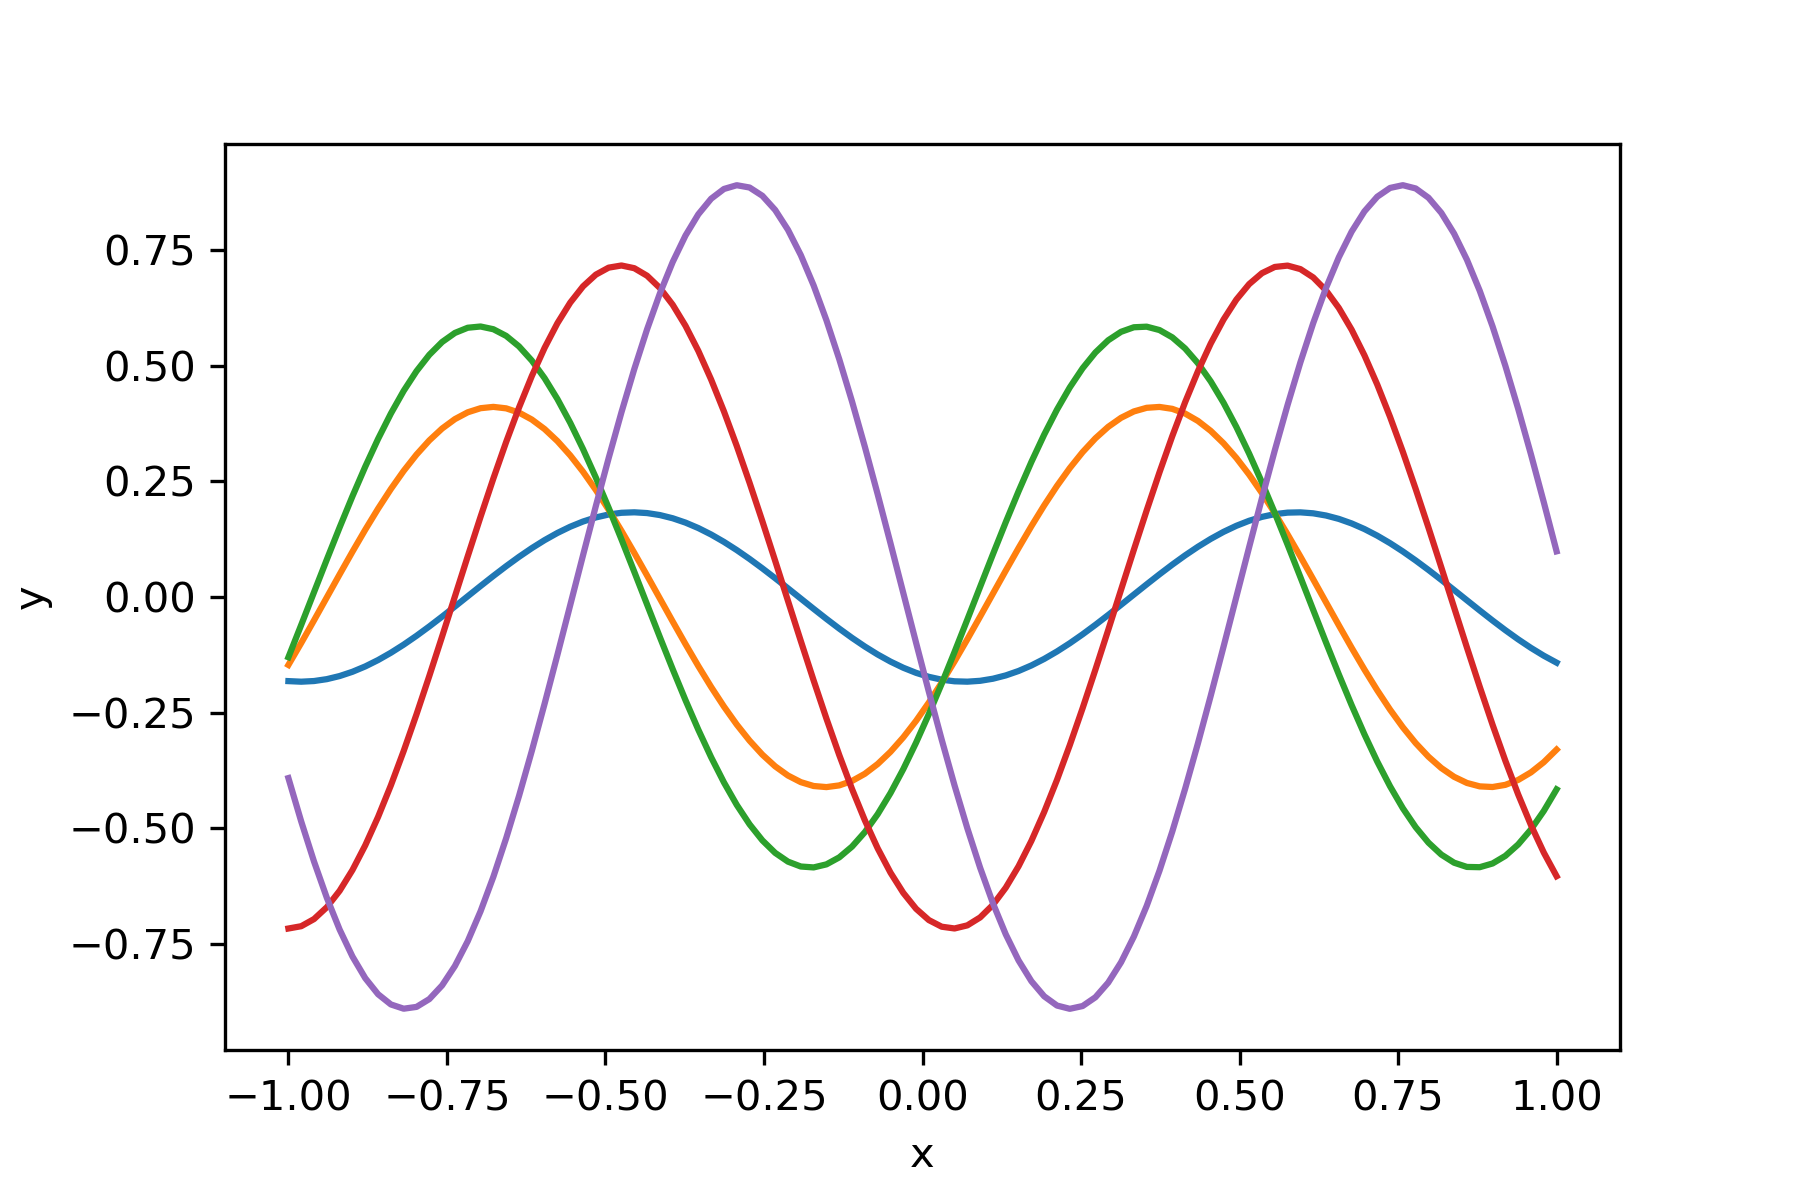
\includegraphics[width=.55\linewidth]{./figs/sinusoidal_functions.png}  
	\caption{$5$ indicative tasks for $\omega = 6$, $x \in [-1, 1]$, $A$ drawn from $Uniform([0.1,1])$ and $s$ drawn from $Uniform([-\pi,\pi])$.}
	\label{}
\end{figure}

\subsubsection{Tanh + sinusoidal functions with varying sharpness}

Tasks are given by 
\begin{equation}
	y = \alpha_1 \tanh(\omega_1 x) + \alpha_2 \sin(\omega_2 x)
\end{equation}
where $\bm{\omega}$, and $\bm{\alpha}$ vary.
\begin{figure}[H]
	\centering
	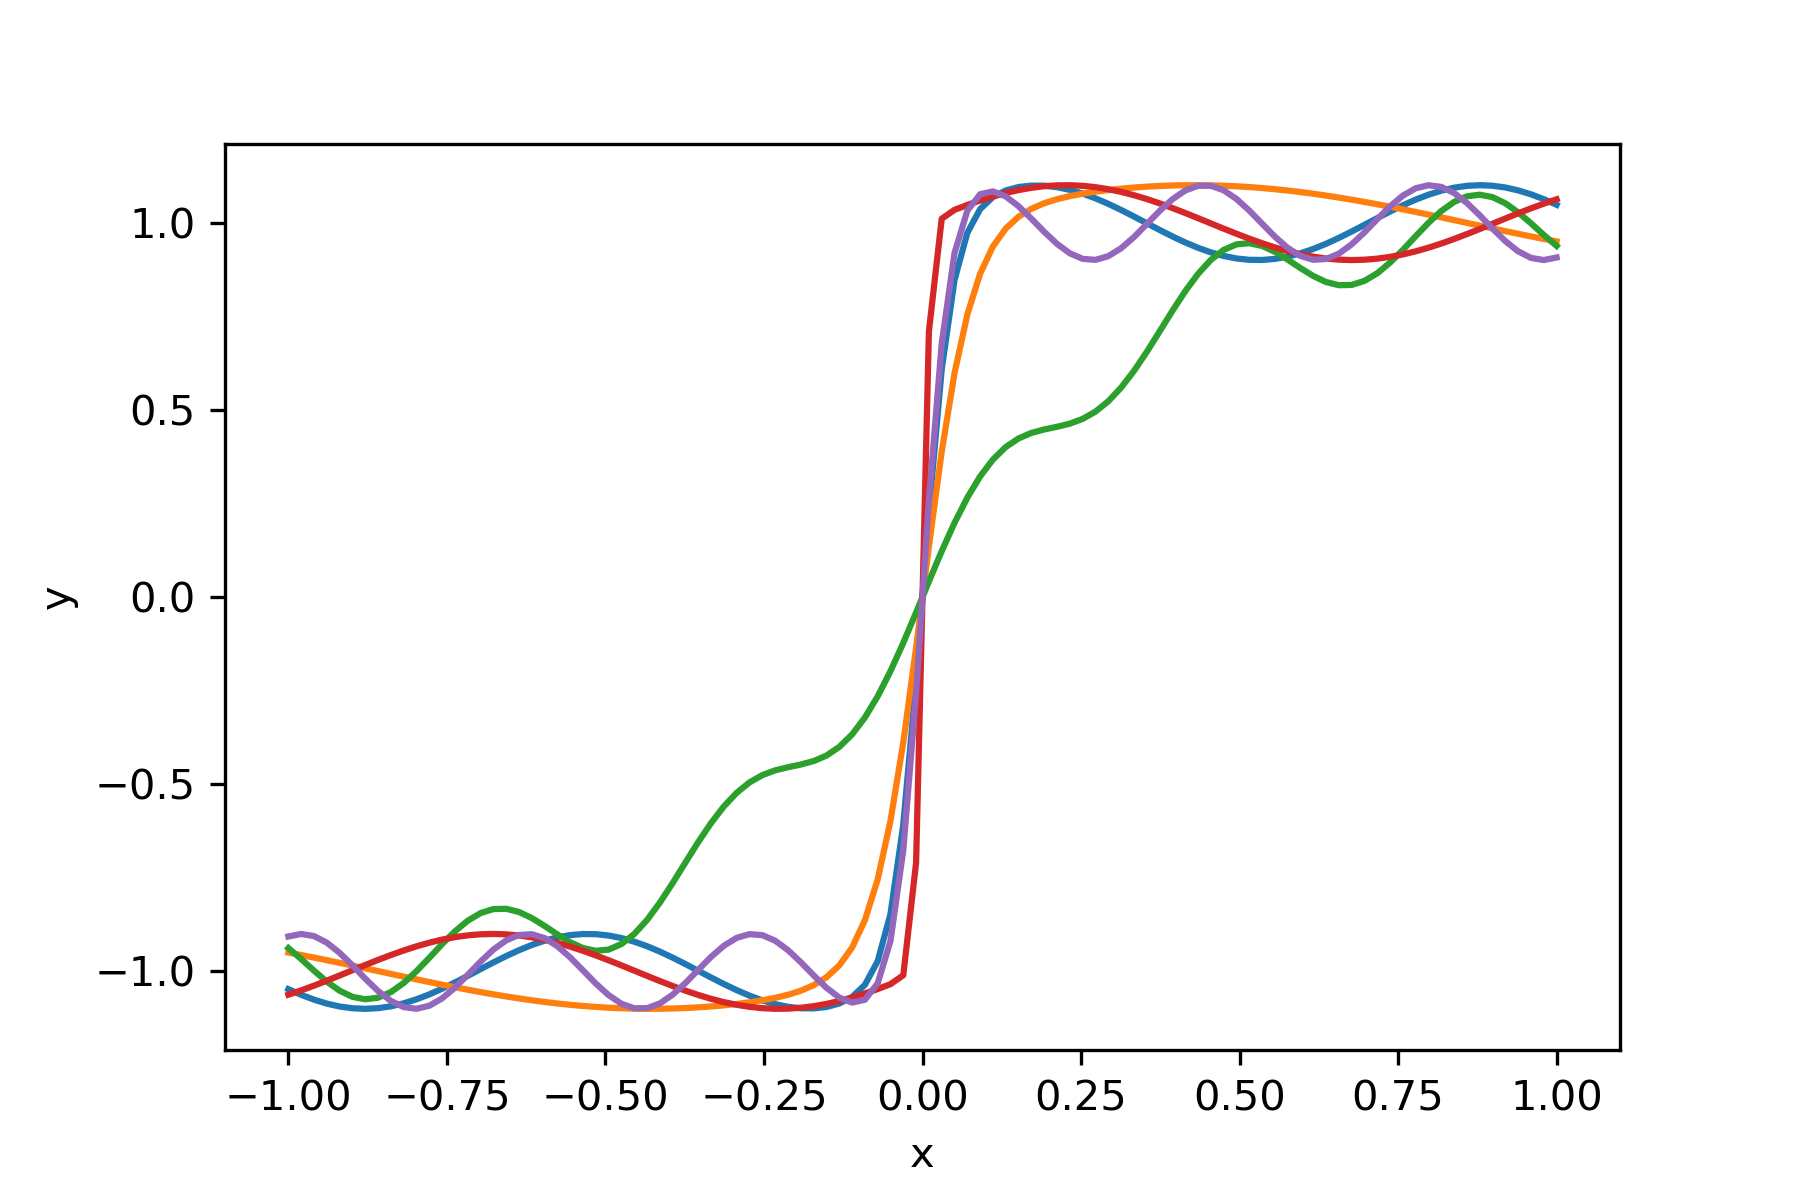
\includegraphics[width=.55\linewidth]{./figs/tanh_plus_sin_functions.png}  
	\caption{$5$ indicative tasks for $x \in [-1, 1]$, $\omega_1$ given by $10^{\omega_1'}$ where $\omega_1'$ is drawn from $Uniform([0,2])$ and $\omega_2$ drawn from $Uniform([1,20])$.}
	\label{}
\end{figure}

\subsection{2D x / 1D y}
\subsubsection{Product of sines with varying frequency}

Tasks are given by 
\begin{equation}
	y = \sin(\omega x_1) \sin(\omega x_2)
\end{equation}
where $\omega$ varies.
\begin{figure}[H]
	\centering
	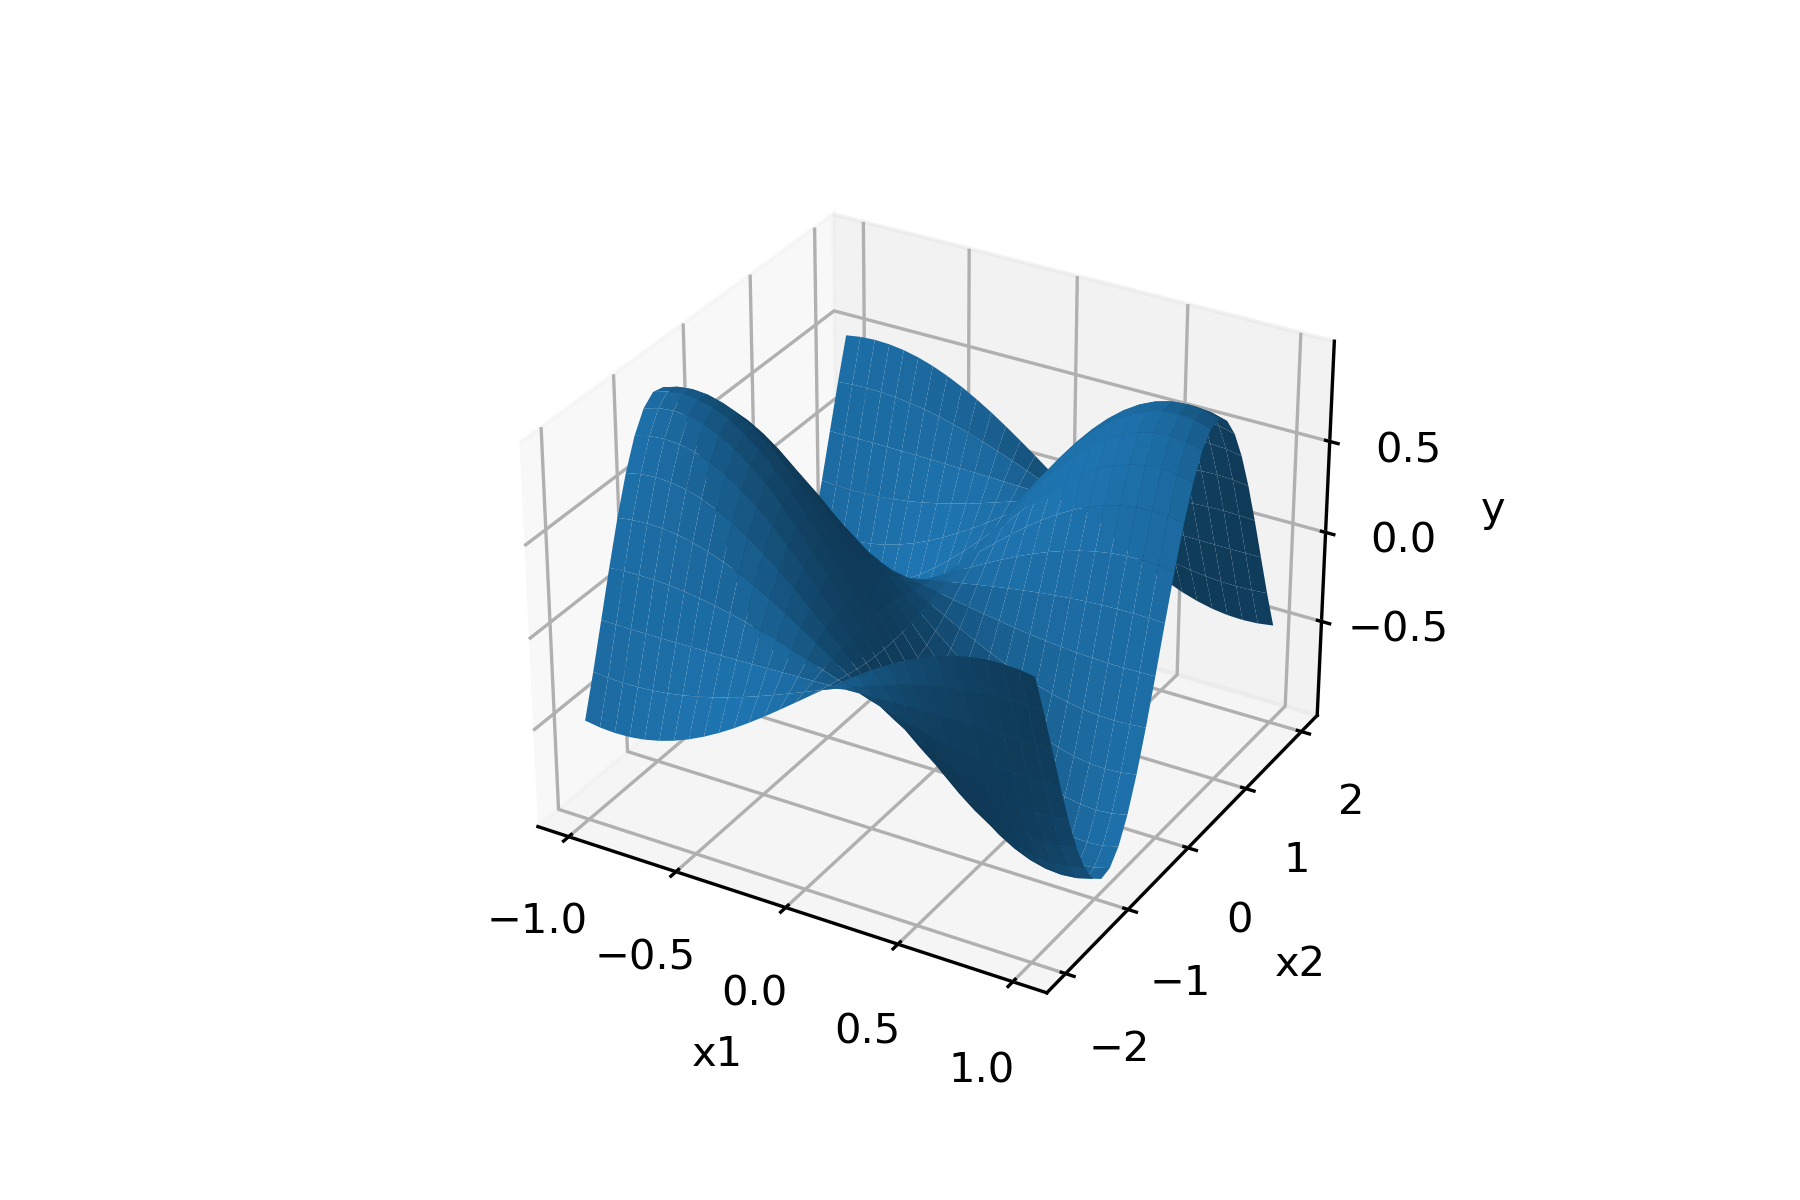
\includegraphics[width=.7\linewidth]{./figs/sinusoidal_product_functions.png}  
	\caption{An indicative task for $x_1 \in [-1, 1]$, $x_2 \in [-2, 2]$, and $\omega$ drawn from $Uniform([1,3])$.}
	\label{}
\end{figure}

\subsection{2D x / 2D y}
\subsubsection{Product of sines and cosines with varying frequencies}

Tasks are given by 
\begin{equation}
	\begin{bmatrix}
		y_1\\y_2
	\end{bmatrix}
	= 	\begin{bmatrix}
		\ sin(\omega_1 x_1) \sin(\omega_1 x_2)\\ \cos(\omega_2 x_1) \cos(\omega_2 x_2)
	\end{bmatrix}
\end{equation}
where $\omega_1$, $\omega_2$ vary.
\begin{figure}[H]
	\centering
	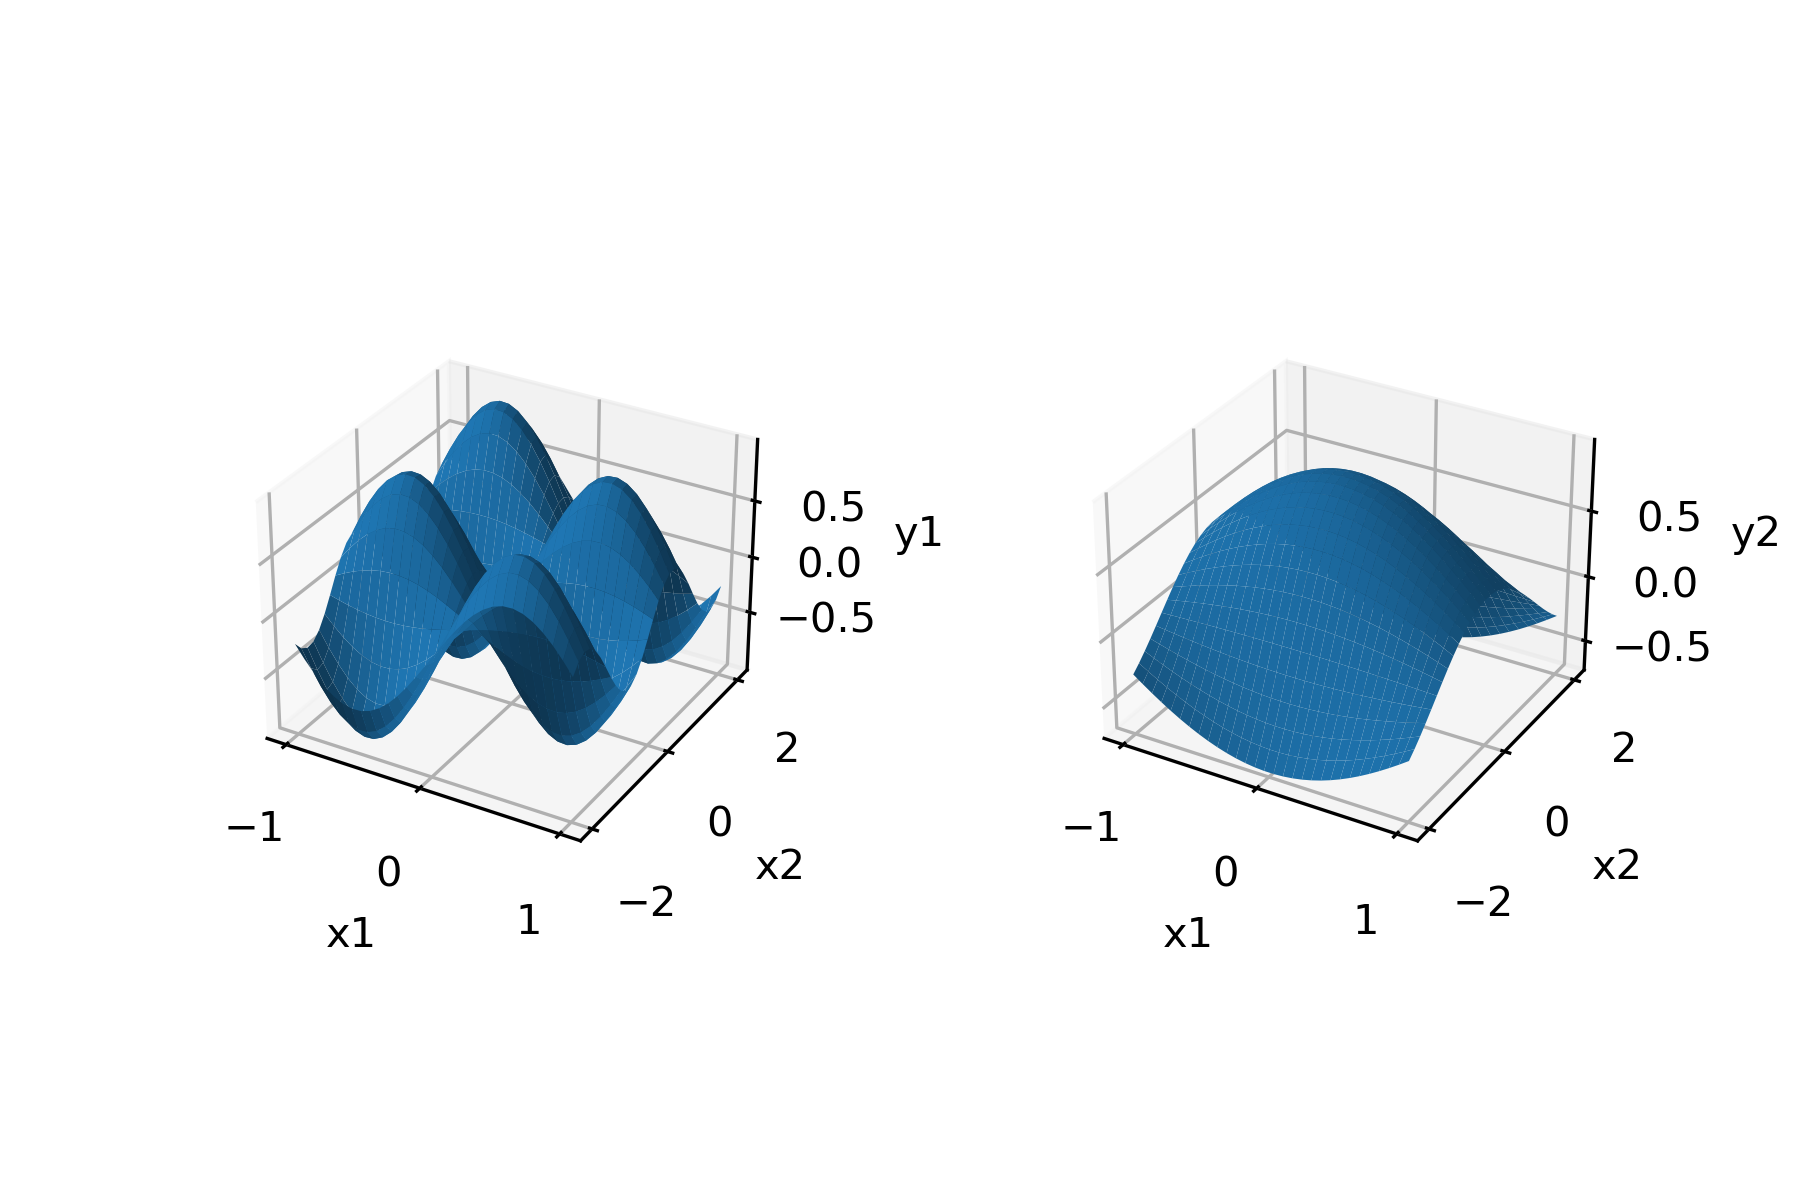
\includegraphics[width=1\linewidth]{./figs/sincos_product_functions.png}  
	\caption{An indicative task for $x_1 \in [-1, 1]$, $x_2 \in [-2, 2]$, and $\omega_1$, $\omega_2$ drawn from $Uniform([1,3])$.}
	\label{}
\end{figure}

%%%%%%%%%%%%%%%%%%%%%%%%%%%%%%%%%%%%%%%%%%%%%%%%%%%%%%%%%%%%%%%%%%%%%%%%%%%%%%%%%%%%%%%%%%%%%%%%%%%%%%%%%	

%\section*{Appendix}
\newpage	
\printbibliography[heading=bibintoc,title={References}]
	
\end{document}